\documentclass[border=3pt,tikz]{standalone}
\usepackage{amsmath} % for \text
\usepackage{tikz}
\tikzset{>=latex} % for LaTeX arrow head
\usepackage{xcolor}
\colorlet{myblue}{black!40!blue}
\colorlet{myred}{black!40!red}
 
\begin{document}
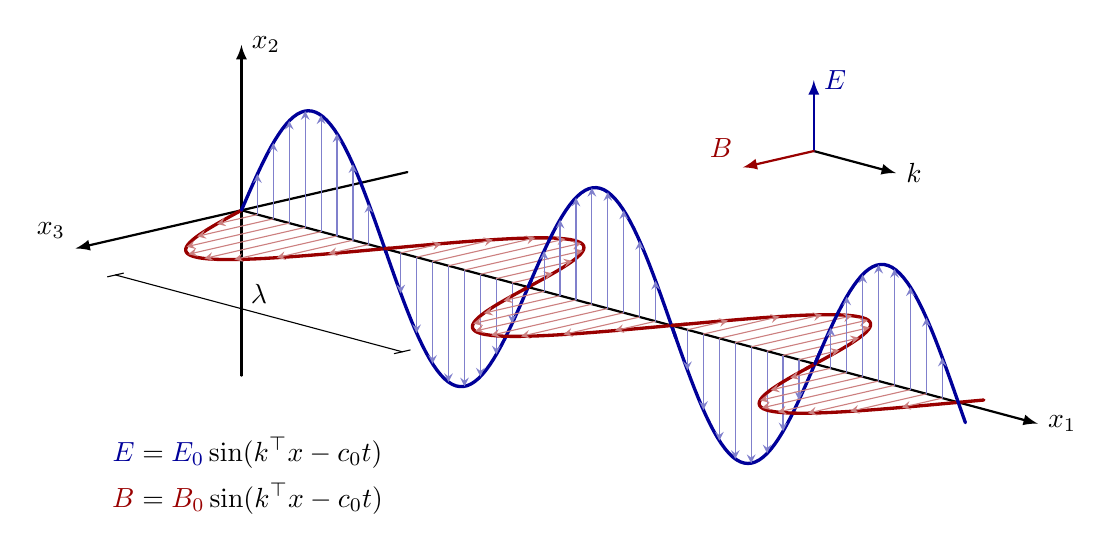
\begin{tikzpicture}[
	x=(-15:1.2), y=(90:1.0), z=(-150:1.0),
        line cap=round, line join=round,
        axis/.style={black, thick,->},
        vector/.style={>=stealth,->}
]
	\def\A{1.5}
	\def\nNodes{5} % use even number
	\def\nVectorsPerNode{8}
	\def\N{\nNodes*40}
	\def\xmax{\nNodes*pi/2*1.01}
	\pgfmathsetmacro\nVectors{(\nVectorsPerNode+1)*\nNodes}

	\def\vE{{\color{myblue}E}}
	\def\vB{{\color{myred}B}}
	\def\vk{k}

	\def\drawENode{ % draw E node and vectors with some offset
		\draw[myblue,very thick,variable=\t,domain=\iOffset*pi/2:(\iOffset+1)*pi/2*1.01,samples=40] plot (\t,{\A*sin(\t*360/pi)},0);
		\foreach \k [
			evaluate={\t=\k*pi/2/(\nVectorsPerNode+1);
			\angle=\k*90/(\nVectorsPerNode+1);}
		] in {1,...,\nVectorsPerNode} {
			\draw[vector,myblue!50]  (\iOffset*pi/2+\t,0,0) -- ++(0,{\A*sin(2*\angle+\iOffset*180)},0);
		}
	}
	\def\drawBNode{ % draw B node and vectors with some offset
		\draw[myred,very thick,variable=\t,domain=\iOffset*pi/2:(\iOffset+1)*pi/2*1.01,samples=40] plot (\t,0,{\A*sin(\t*360/pi)});
		\foreach \k [
			evaluate={\t=\k*pi/2/(\nVectorsPerNode+1);
			\angle=\k*90/(\nVectorsPerNode+1);}
		] in {1,...,\nVectorsPerNode} {
			\draw[vector,myred!50]  (\iOffset*pi/2+\t,0,0) -- ++(0,0,{\A*sin(2*\angle+\iOffset*180)});
		}
	}

	% main axes
	\draw[axis] (0,0,0) -- ++(\xmax*1.1,0,0) node[right] {$x_1$};
	\draw[axis] (0,-\A*1.4,0) -- (0,\A*1.4,0) node[right] {$x_2$};
	\draw[axis] (0,0,-\A*1.4) -- (0,0,\A*1.4) node[above left] {$x_3$};

	\draw (pi/4, 0, 2.4) -- ++(0, 0, 0.2);
	\draw (pi + pi/4, 0, 2.4) -- ++(0, 0, 0.2);
	\draw (pi/4, 0, 2.5) -- ++(pi, 0, 0) node [midway, above] {\( \lambda \)};
	% small axes
	\def\xOffset{{(\nNodes-2)*pi/2}}
	\def\yOffset{\A*1.2}
	\def\zOffset{\A*1.2}
	\draw[axis,black] (\xOffset,\yOffset,-\zOffset) -- ++(\A*0.6,0,0) node[right,align=center] {$k$}; %\\propagation
	\draw[axis,myblue]  (\xOffset,\yOffset,-\zOffset) -- ++(0,\A*0.6,0) node[right] {$E$};
	\draw[axis,myred]   (\xOffset,\yOffset,-\zOffset) -- ++(0,0,\A*0.6) node[above left] {$B$};
	% equation
	\node[above right] at (\xOffset,-0.5*\yOffset,4*\zOffset)
	{$%
		\begin{aligned}
			\vE &= {\color{myblue} E_0}\sin(\vk^\top x - c_0t)\\
			\vB &= {\color{myred} B_0}\sin(\vk^\top x - c_0t)\\
		\end{aligned}%
	$};
	% draw (anti-)nodes
	\foreach \iNode [evaluate={\iOffset=\iNode-1;}] in {1,...,\nNodes}{
		\ifodd\iNode \drawBNode \drawENode % E overlaps B
		\else        \drawENode \drawBNode % B overlaps E
		\fi
	}
\end{tikzpicture}
\end{document}
